\chapter{System Design}
\section{The Database}
The MySQL database is the core foundation of Repota. The database stores workers, sessions, job reports (service report) and customer details in their own respected tables. In the database everything is connected to a worker. 

\subsubsection{Workers \& Session}
The workers table is in relation of a users table and consists of a worker\_id, user\_name, worker\_name and a hash (password). The ID is set up to be automatically incremented, meaning when a new worker is inserted to the table an ID does not have to be specified. Their username is set as unique to avoid data collisions with other workers in the database. Their worker name is set as as the unique key as this name is to be presented with all their reports on the front-end. Their ID connects them to the session table making it a foreign key. Here the session ID is set up to be a UUID (Universally Unique ID). An expiry time field is setup for user's login sessions. The session ID and expiry time are also used as the requirements for browser cookies.

\subsubsection{Job Reports \& Customers}
Workers are connected to their reports by their ID making this a foreign key for the jobreports table. The report's ID is a foreign for the customers table. The jobreports table holds quite a bit of information. This information is split into fourteen fields. The customers table consists of a customer\_id, job\_report\_id (foreign key), customer\_name and customer\_complaint.  The following describes how the tables; workers, jobreports and customers all link together. 
\newpage
\subsubsection{Full Report Details}
A full report (Figure 4.1) required a lot of information which is in sixteen components. Meaning the information had to spread out between tables to have them all still link to the workers and customers to avoid one large table and still keep the workers and session table intact. All this information is obtained by quite a large JOIN Query (Figure 4.2).

\begin{figure}[H]
    \caption{Example of a Full Report}
    \label{image:dbReport}
    \centering
    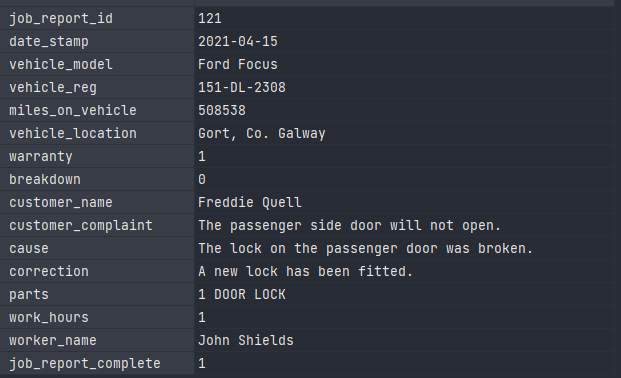
\includegraphics[width=0.8\textwidth]{images/database/job_report.png}
\end{figure}

\begin{figure}[H]
    \caption{JOIN QUERY  for all Report information}
    \label{image:join}
    \centering
    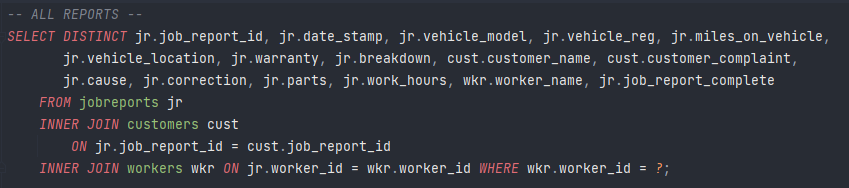
\includegraphics[width=1.0\textwidth]{images/database/raw_mysql_join.png}
\end{figure}

\subsubsection{Refactoring}
The first refactor was due to duplicate results coming from JOIN QUERYs. Even though the data was unique the query had trouble selecting all the report's data. The report IDs were then altered to be drastically different having them is the hundreds instead of '1-2-3-4-5' and the duplicate problem was solved. The jobreports table was originally split into two tables, jobreports, and workdone. When it came to implementing the CRUD operations in the back-end, it made a lot more sense to have this information in one table as it would have made for some monstrous queries for updating and creating. In the old jobreports table, the fields warranty and breakdown were originally varchars for a simple "YES" or "NO". With this refactoring, these fields were changed to booleans along with the addition of 'job\_report\_complete' to allow workers to keep track of their complete and incomplete reports. The figure below shows the finalized database design.

\begin{figure}[H]
    \caption{Database Schema}
    \label{image:db}
    \centering
    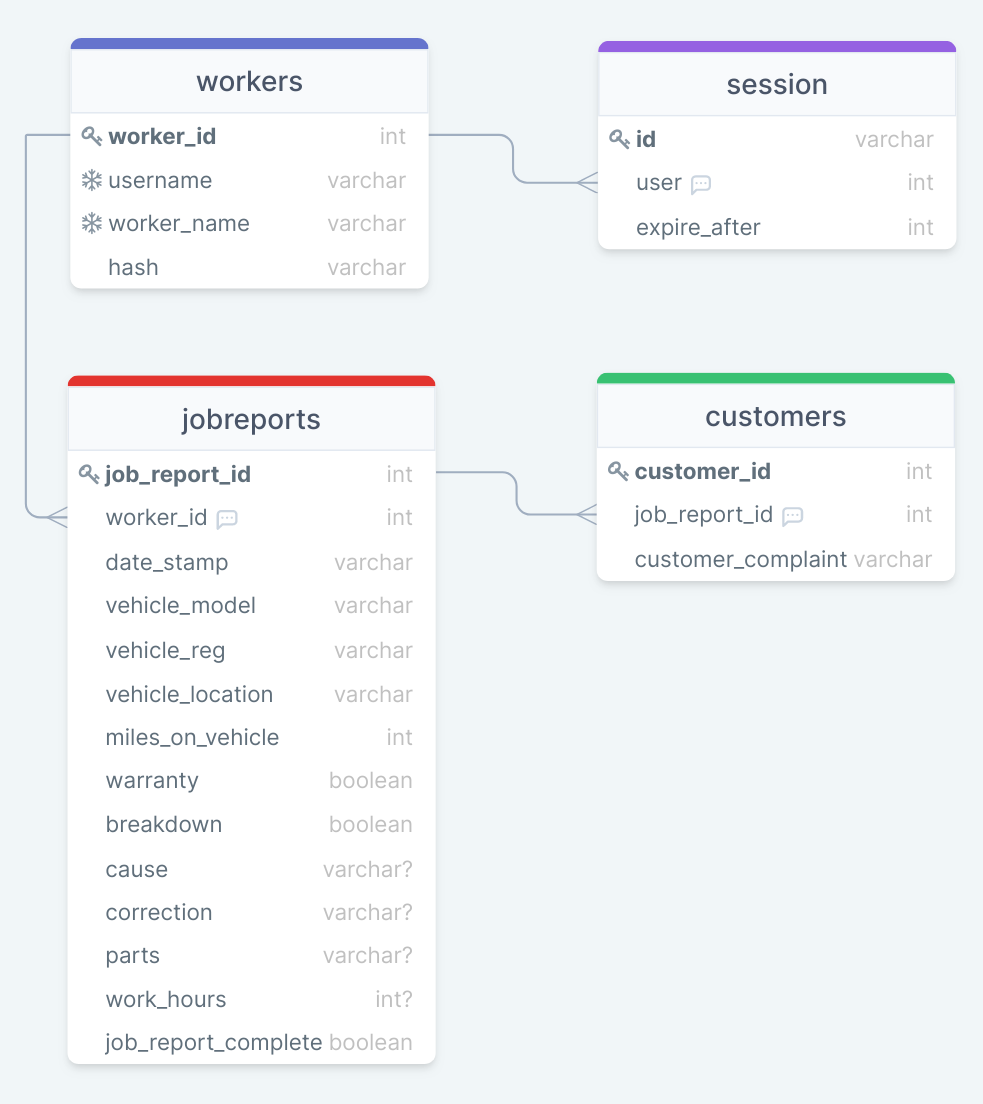
\includegraphics[width=0.8\textwidth]{images/database/database.png}
\end{figure}

\subsection{Database Hosting}
The database is hosted on an AWS EC2 Ubuntu Virtual Machine as a server. This provides a virtual private cloud (VPC) with transmission control protocol (TCP) for ports 22 (SSH login (Secure Shell)) and 3306 (MySQL). This holds the database in a secure environment, which only the back-end has access to through a configuration file with the MySQL details. Therefore the data on workers, reports and customers are kept safe. The figure below shows the entire set of the server.

\begin{figure}[H]
    \caption{EC2 Ubuntu Server}
    \label{image:db_aws}
    \centering
    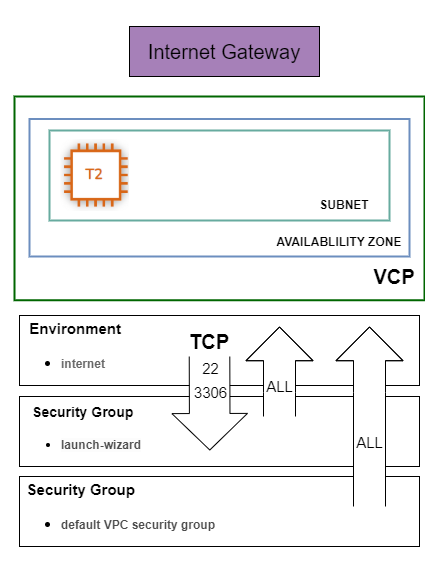
\includegraphics[width=1.0\textwidth]{images/aws/aws_linux.png}
\end{figure}

\newpage
\section{The Back-end}
Repota depends on the robust and quick back-end nicknamed 'Horton'. 
Horton handles all user registration, login, logout, sessions, report CRUD operations, and has access to a 3rd Party API named 'Back4App' for vehicle information. Without him Repota would be quite limited in terms of the service it provides. 

\subsection{Horton API Specification}
Horton's API specification was designed using the OpenAPI tools from Swagger and is written in YAML. The specification design consists of RESTful routes, operationIds, HTTP methods, status codes and schema models. 
The specification worked as a prototype to set up the necessary functions and data models for users and their reports. 
Swagger provided HTML documentation of Horton's specification. This documentation was extremely useful for when it came to implement the main features. The documentation is hosted using GitHub pages. This was mainly to provide easy access. However it can be useful to other developers if they require to develop an API for a service report app or even for a user account system. The documentation displays the API's operations, login, register, createReport, deleteReport, getReportbyId, getReports and updateReport. It also provides code samples for said operations with an example of a response HTTP status code and message. Schema Models are also presented to show the data required in them. The documentation URL is provided below.
\\\\ Horton API Documentation: \\ 
\url{https://johnshields.github.io/horton.api.doc/}

\subsubsection{Operations}
In OpenAPI specification, operations are identified by operationIds which is a unique string identifier. These operations are templates of CRUD operations with HTTP methods, e.g., POST, GET, DELETE, PUT. Operations contain tags, a description, parameters such as an ID, a request body for data, a response status, headers, login requirements and a URL. The user account system and report system were both designed initially as operationIds with their respected paths. Figure 4.5 shows how the login operation was designed. All these operations provided the necessary templates for the handler functions of each path. 

\begin{figure}[H]
    \caption{Login Operation}
    \label{image:operationId}
    \centering
    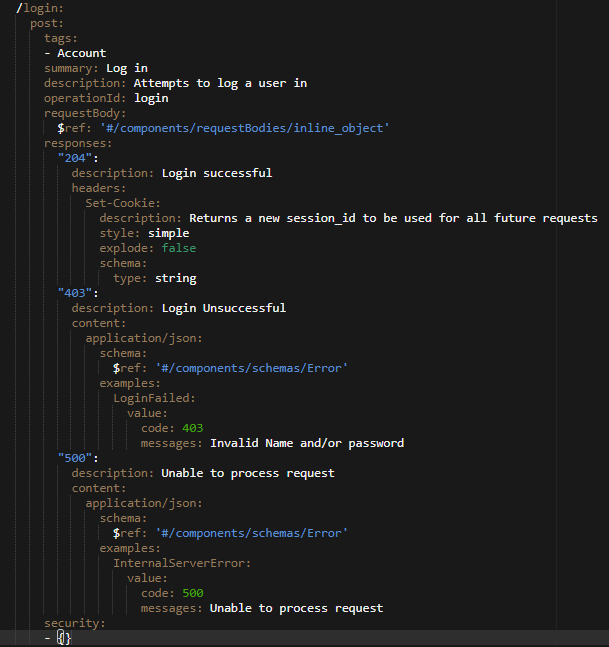
\includegraphics[width=0.8\textwidth]{images/open_api/login-spec.png}
\end{figure}

\subsubsection{RESTful Routes}
Horton's designed routes consist of two paths for user registration and login. For CRUD operations on reports there are five paths (Figure 4.6). These paths provided structure for the API and for HTTP methods.

\subsubsection{Schema Models}
Figure 4.7 shows the finalized models that were designed to represent user details, status codes with messages and reports. Implementing the API’s design resulted in refactoring the initial models designed to accommodate the databases changes and an addition of three other routes for a logout, a 3rd Party API and an Index Handler, which will be discussed in the next section.

\begin{figure}[!ht]
    \caption{API Paths}
    \label{image:paths}
    \centering
    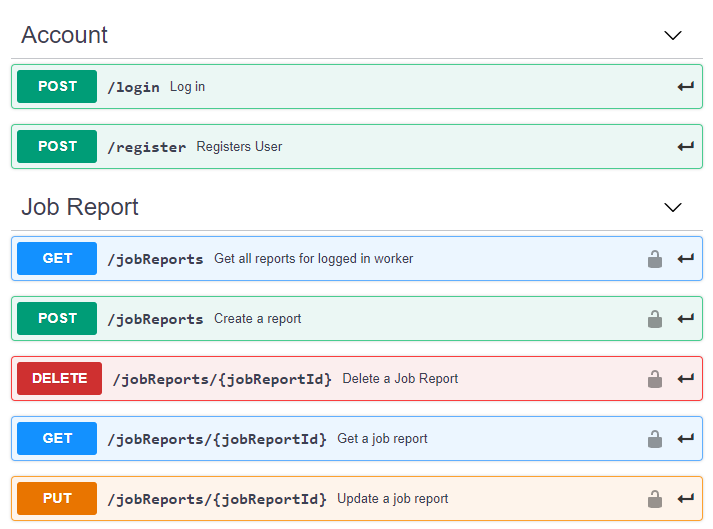
\includegraphics[width=1.0\textwidth]{images/open_api/paths.png}
\end{figure}

\begin{figure}[H]
    \caption{Schema Models}
    \label{image:models}
    \centering
    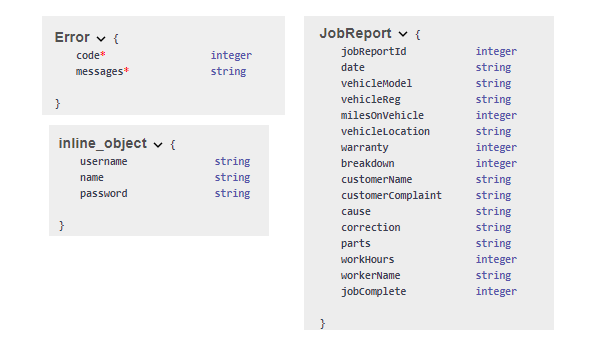
\includegraphics[width=1.0\textwidth]{images/open_api/shema_models2.png}
\end{figure}

\subsection{Go Horton}
Horton himself is written in Go using the web framework Gin Gonic to design and implement him into a robust API. When the API specification had the core fundamentals, it was time to generate the prototype code stubs. Swagger does not provide an option for Gin; this resulted in using another OpenAPI generator with Docker. This prototype set up the necessary functions for registration, login, and all report CRUD operations. The remainder of this section conveys how the final product has come a long way from these generated stubs.

\subsubsection{Database Connection}
The MySQL database connection is made in db\_connection.go with the function DbConn. The MySQL details are loaded from a configuration (config) file then a MySQL driver is opened with the details for access to the database. The config file is to be sure the database details are kept safe and not exposed. Errors are handled for loading the config and the MySQL driver connection to ensure the failure of a database connection is alerted. 

\begin{figure}[H]
    \caption{DbConn Function}
    \label{image:DbConn}
    \centering
    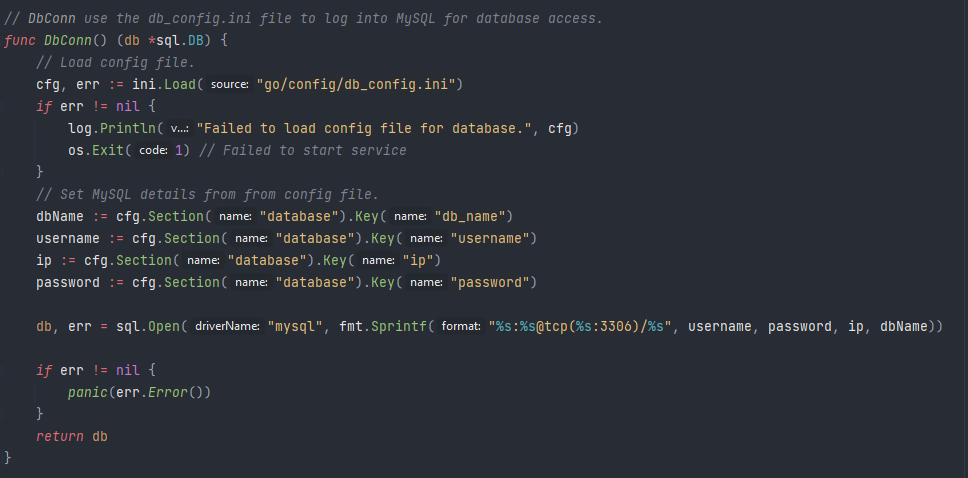
\includegraphics[width=1.0\textwidth]{images/horton/db_conn.png}
\end{figure}
 \newpage
\subsubsection{Data Models}
The data models from the API specification, 'InLineObject' and 'JobReport', required some light refactoring to avoid completely generating the stubs again. InLineObject is for new users in the system. This model now consists of a username, name and password. The name is now included as for the reports required a name to be displayed with all the other details. For the JobReport model, 'Warranty', 'Breakdown' and the addition of 'JobComplete' were all set as int values (to accommodated the database changes of booleans) to allow them to be check-box values on the front-end. New models were created for login sessions and a 'worker account'. These models are used to send and receive JSON data to/from the front-end. See the figures below for the Go Structs of the finalized models. 

\begin{figure}[H]
\begin{minipage}[b]{0.45\linewidth}
    \centering
    \caption{InLineObject Struct}
    \label{image:inLineObjectStruct}
    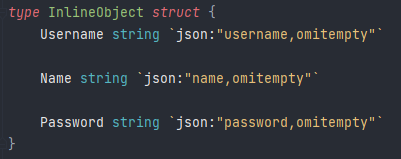
\includegraphics[width=1.0\textwidth]{images/horton/models/inlineobject_stuct.png}
    \caption{Session Struct}
    \label{image:sessionStruct}
    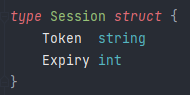
\includegraphics[width=0.8\textwidth]{images/horton/models/session_struct.png}
    \caption{WorkerAccount Struct}
    \label{image:workerStruct}
    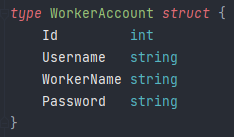
\includegraphics[width=0.8\textwidth]{images/horton/models/worker_stuct.png}
\end{minipage}
\quad
\begin{minipage}[b]{0.45\linewidth}
    \caption{JobReport Struct}
    \label{image:reportStruct}
    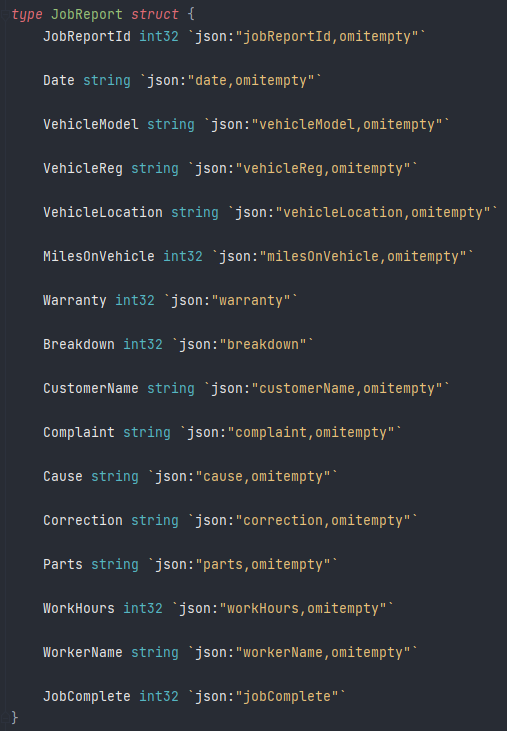
\includegraphics[width=1.0\textwidth]{images/horton/models/report_struct.png}
\end{minipage}
\end{figure}

\subsubsection{Routers}
The API now includes ten paths which each have their respected handler functions.
These paths are all managed in routers.go. The API's main function boots up these 'routers' after the essential CORS requirements have been set (Figure 4.13). Table 4.1 displays the handler functions and their paths.  

\begin{figure}[H]
    \caption{CORS function}
    \label{image:cors-req}
    \centering
    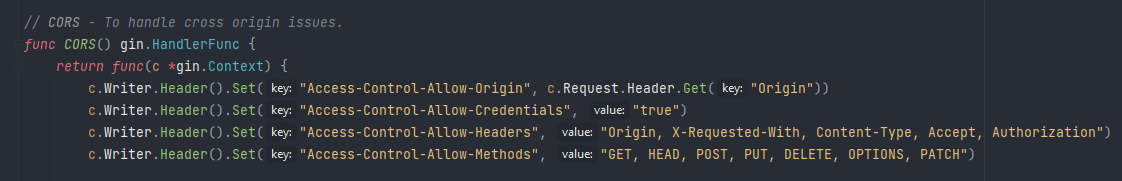
\includegraphics[width=1.0\textwidth]{images/horton/cors.png}
\end{figure}

\begin{table}[H]
\caption{Handler functions \& their paths}
\begin{tabular}{|l|l|l|}
\hline
Function      & HTTP request \& path         & Description            \\ \hline\hline
Index         & GET /api/v1/                 & Index                  \\ \hline
Register      & POST /api/v1/register        & User Registration      \\ \hline
Login         & POST /api/v1/login           & User Login             \\ \hline
Logout        & GET /api/v1/logout           & User Logout            \\ \hline
CreateReport  & POST /api/v1/jobReports      & Create a Report        \\ \hline
DeleteReport  & DELETE /api/v1/jobReports/ID & Delete a Report        \\ \hline
GetReportById & GET /api/v1/jobReports/ID    & Get a Report           \\ \hline
GetReports    & GET /api/v1/jobReports       & Get all Reports        \\ \hline
UpdateReport  & PUT /api/v1/jobReports/ID    & Update a Report        \\ \hline
GetCarApiData & GET /api/v1/carApiData       & Get data from Back4App \\
\hline
\end{tabular}
\end{table}

The following sections will go into detail on how the handler functions work with their paths and models.

\subsection{Account \& Session System}
\subsubsection{Registration}
When a user registers, they become a 'worker' as the app is revolved around a work environment. Users POST a request to register by their username, name, and password which relies on the InLineObject model. The user's username and name are checked with the function isValidAccount to ensure they do not already exist. The password gets hashed using Go's package 'bcrypt', which implements the Provos and Mazières's bcrypt adaptive hashing algorithm. \cite{ref25} After the details check and the password hashing, the new user is inserted into the database, and a session ID (token) is generated with the Session model and is inserted into the database for them (Figures 4.14-4.18). Once a user is in the database, they are uniquely identified by their worker ID. This ID is also attached to their session in the database (Figure 4.19). This session is designed for Cookies to let the user make all future requests to the API.

\begin{figure}[H]
\begin{minipage}[b]{0.6\linewidth}
    \centering
    \caption{Register}
    \label{image:regFunc}
    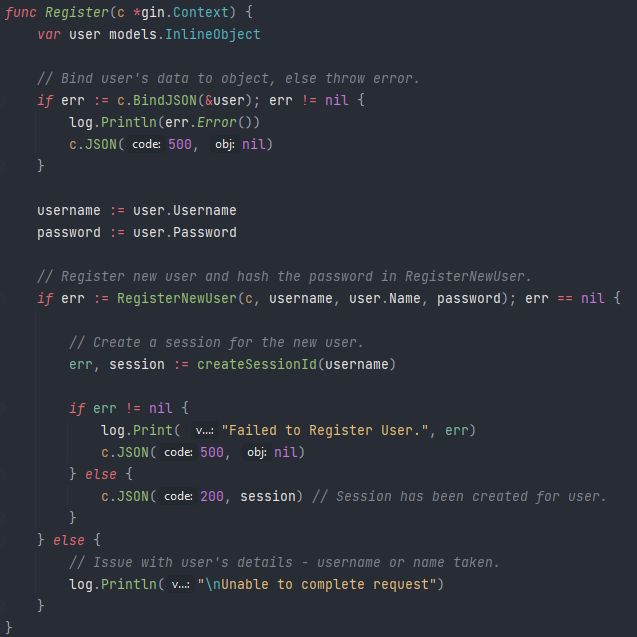
\includegraphics[width=1.0\textwidth]{images/horton/account_system/register_func.png}
    \caption{RegisterNewUser}
    \label{image:regUserFunc}
    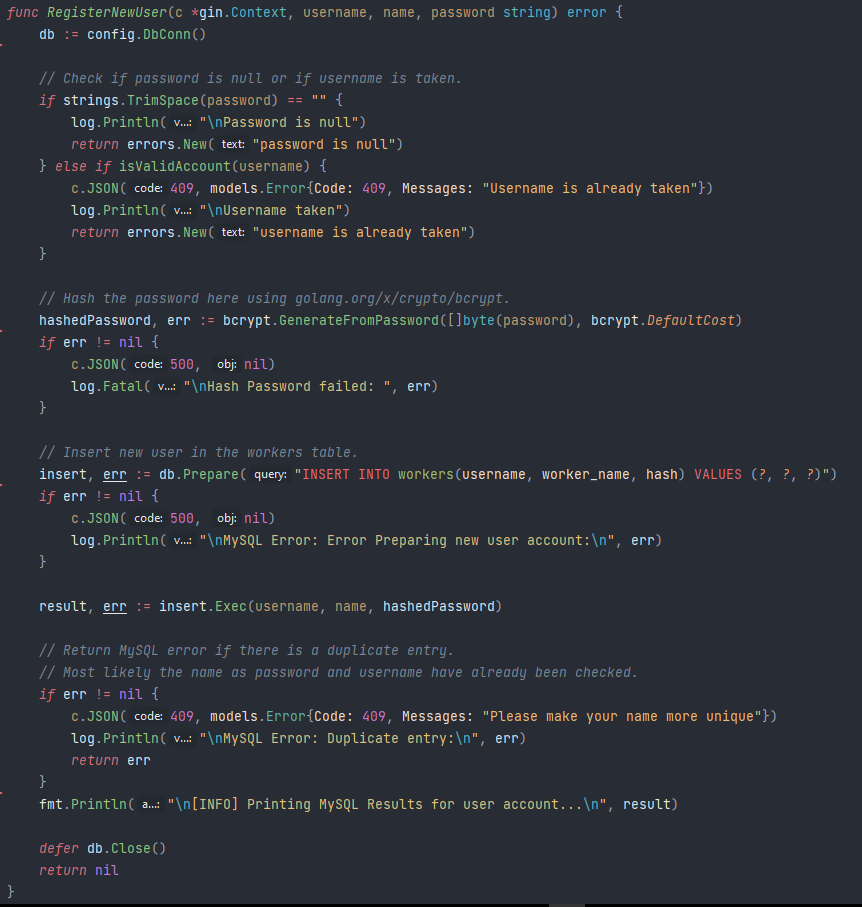
\includegraphics[width=1.0\textwidth]{images/horton/account_system/register_new_user.png}
\end{minipage}
\quad
\begin{minipage}[b]{0.6\linewidth}
    \caption{isValidAccount}
    \label{image:validAccount}
    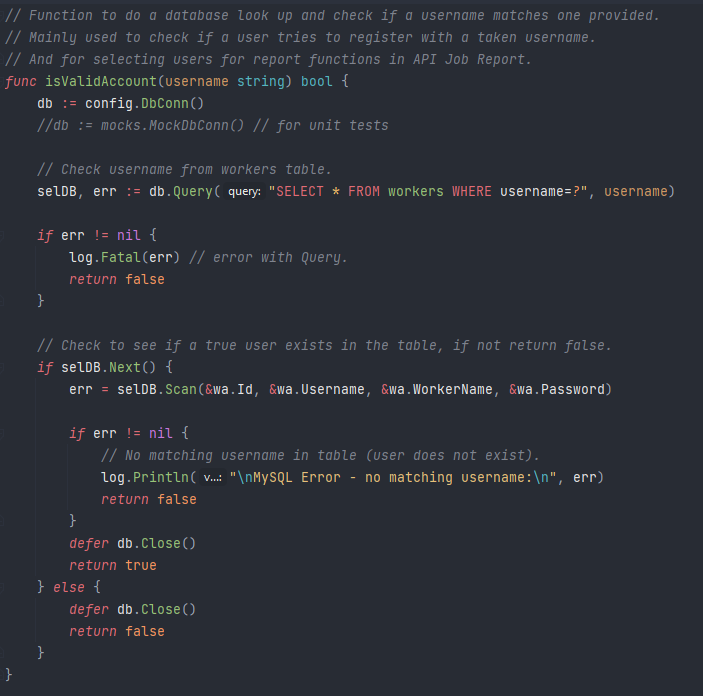
\includegraphics[width=1.0\textwidth]{images/horton/account_system/valid_account_func.png}
    \caption{createSessionId}
    \label{image:createSession}
    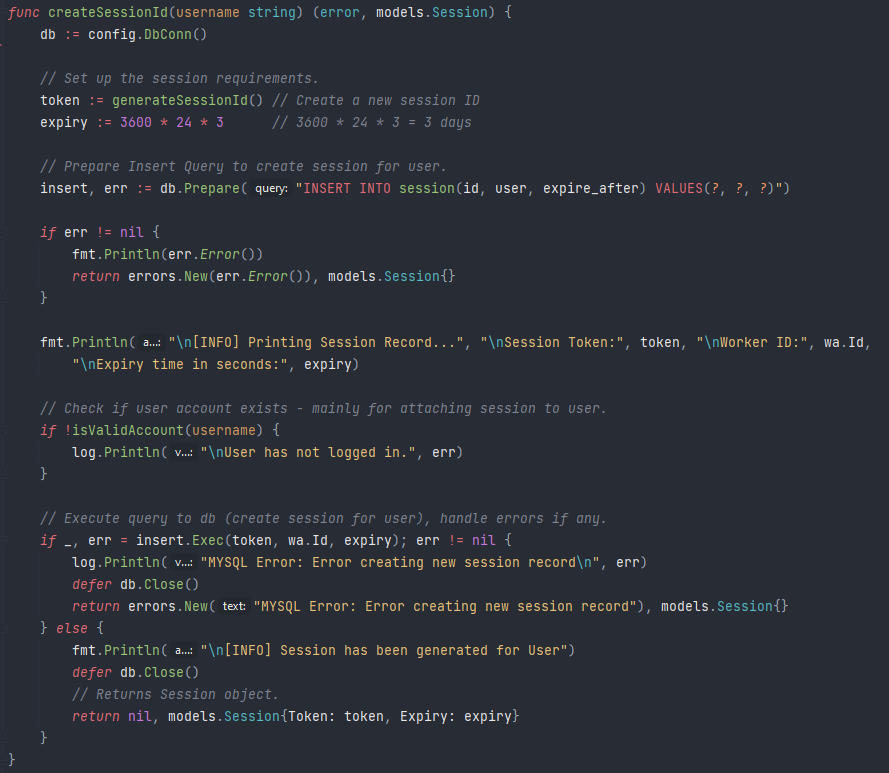
\includegraphics[width=1.0\textwidth]{images/horton/account_system/create_session.png}
    \caption{generateSessionId}
    \label{image:genSession}
    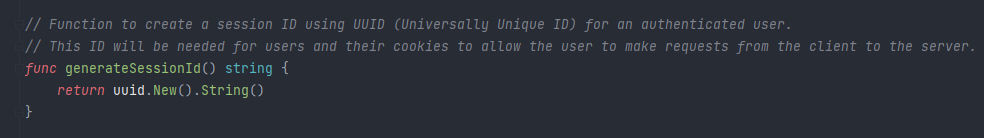
\includegraphics[width=1.0\textwidth]{images/horton/account_system/generate_session.png}
\end{minipage}
\end{figure}
 
\begin{figure}[H]
    \caption{User in the workers and session tables}
    \label{image:userinDb}
    \centering
    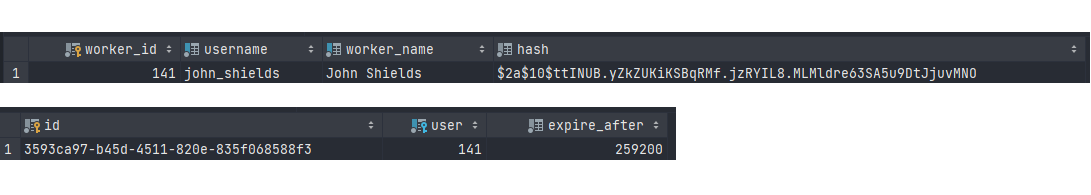
\includegraphics[width=0.8\textwidth]{images/database/usr_In_db.png}
\end{figure}

\subsubsection{Login}
A user logs in by their username and password which works with the WorkerAccount model. This data gets sent through a POST request that checks to see if the username exists in the database, then hashes the entered password and compares it to the one in the database. If the user has an existing session that one is removed and replaced by a new one. If their details are correct and the new session has been created, a cookie of three days is set for them then, the user has been logged in successfully (Figures 4.20-4.22).

\begin{figure}[H]
\centering
\begin{minipage}[b]{0.6\linewidth}
    \centering
    \caption{Login}
    \label{image:login}
    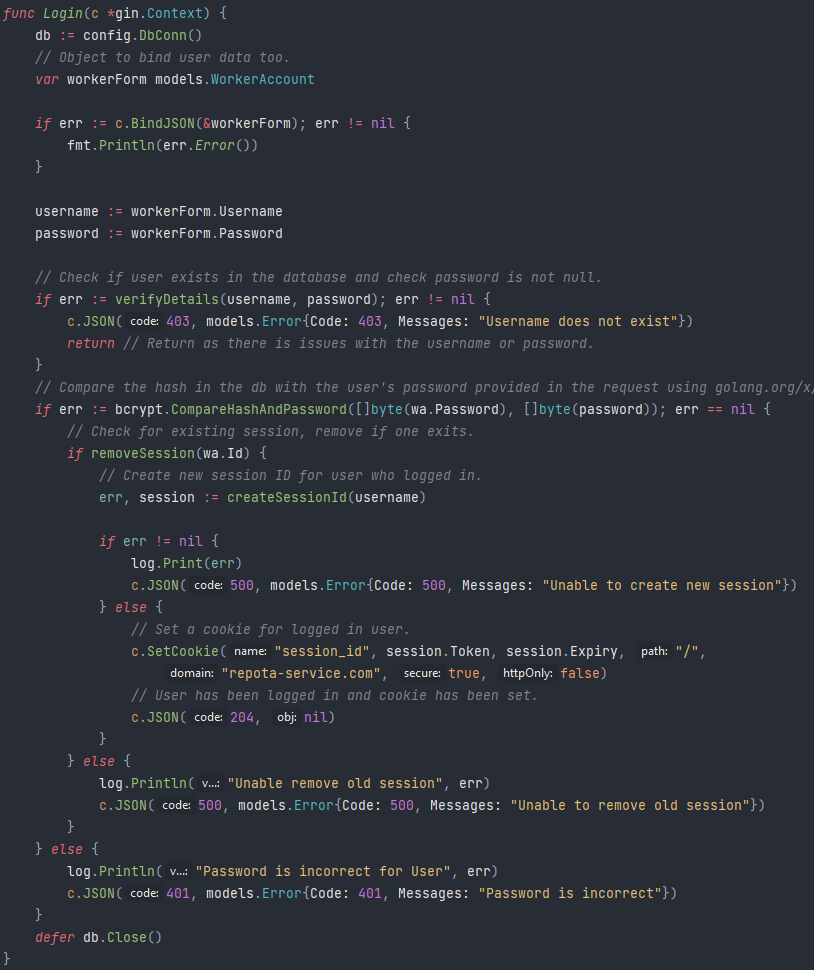
\includegraphics[width=1.0\textwidth]{images/horton/account_system/login_func.png}
\end{minipage}
\quad
\begin{minipage}[b]{0.6\linewidth}
    \centering
    \caption{verifyDetails}
    \label{image:verify}
    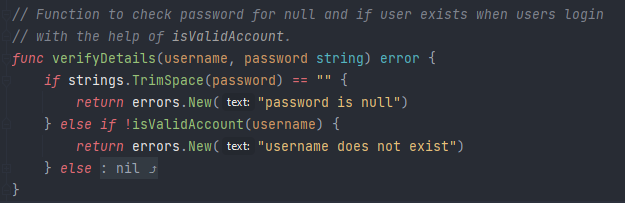
\includegraphics[width=0.9\textwidth]{images/horton/account_system/verifyDetails.png}
\end{minipage}
\end{figure}
 
\begin{figure}[H]
    \centering
    \caption{Browser Cookie}
    \label{image:cookie}
    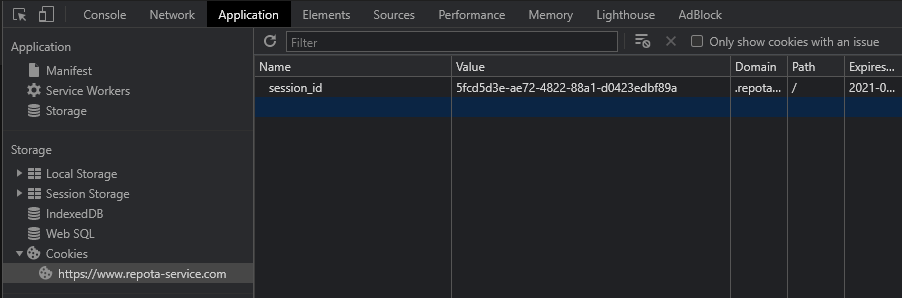
\includegraphics[width=0.9\textwidth]{images/horton/account_system/cookie.png}
\end{figure}

\subsubsection{Logout}
A user is logged out by removing their current session and replacing it with a new one. The new session is set to expire after one second. A new cookie is then set for the user with this session, and then the user is logged out after the cookie expires the one second (Figure 4.23). This was mainly to accommodate how browser cookies work. Only users have control of removing their cookies, and setting a new cookie of one second was the best way to log them out as a user requires a cookie to make all report requests to the API. In the session controller, there is a function for cookie checking (Figure 4.24). The purpose of this function is to block requests on reports if a user have no cookie. In other words an unauthorized user.

\begin{figure}[H]
    \caption{Logout}
    \label{image:logout}
    \centering
    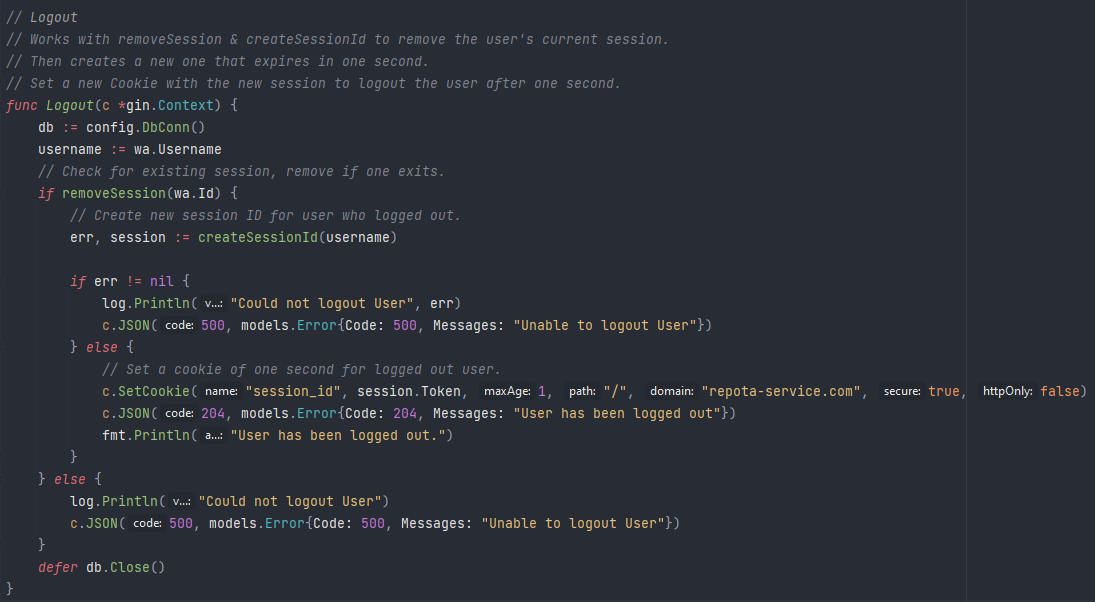
\includegraphics[width=1.0\textwidth]{images/horton/account_system/logout_func.png}
\end{figure}

\begin{figure}[H]
    \caption{CheckForCookie}
    \label{image:cookieCheck}
    \centering
    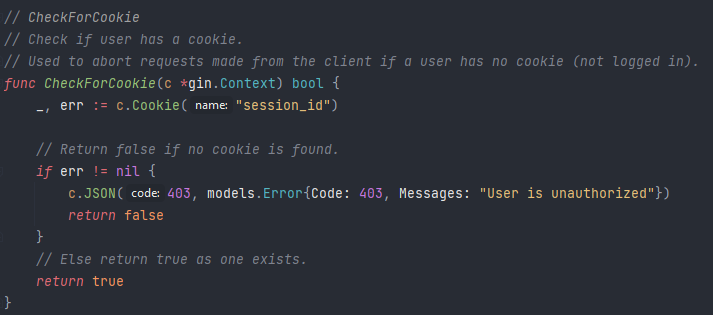
\includegraphics[width=0.8\textwidth]{images/horton/account_system/check_cookie.png}
\end{figure}

Please view the figure below for an overview of how the account and session system works with the controllers, handler functions, HTTP methods, and paths.
\begin{figure}[H]
    \caption{Account System}
    \label{image:accountSystem}
    \centering
    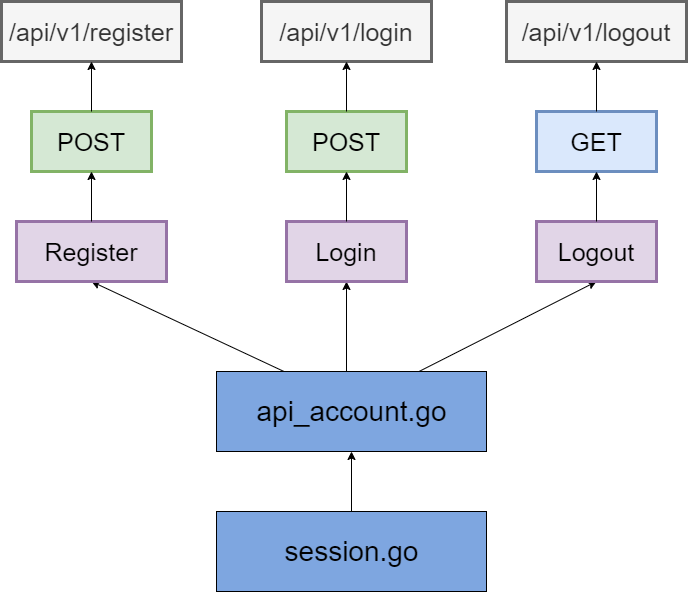
\includegraphics[width=1.0\textwidth]{images/horton/account_system/account_system.png}
\end{figure}

\subsection{Report System}
Users are required to be logged in for all the report operations. This requirement is ensured with the CheckForCookie function shown above. Before each function gets involved with the database, the user is checked for a cookie. If they have one, the function request continues; if they do not, it is aborted.

\subsubsection{Create A Report}
Creating a report is handled by the functions, CreateReport, CheckForCookie, InsertJobReport
and isValidAccount. The process begins with a POST request from the client (front-end) of a new report with the information bound as JSON data with the JobReports. Then the CheckForCookie function comes in, and if that checks out, InsertJobReport is called with the new report data as a parameter along with the user's username and one for Gin to handle status codes (Figure 4.26). The data is then prepared as MySQL INSERT QUERIES for the tables: jobreports and customers in the database (Figure 4.27). Once these are in place, the user is again checked with isValidAccount. This second check is mainly to have the user's 'worker name' in the report's details. Next, a MySQL transaction is begun to execute the INSERTs into the two tables (Figure 4.28). Once the transaction is committed, a new report has been successfully created and a status code of 201 is sent to inform the client it was created. 

\begin{figure}[H]
    \caption{CreateReport Function}
    \label{image:createReport}
    \centering
    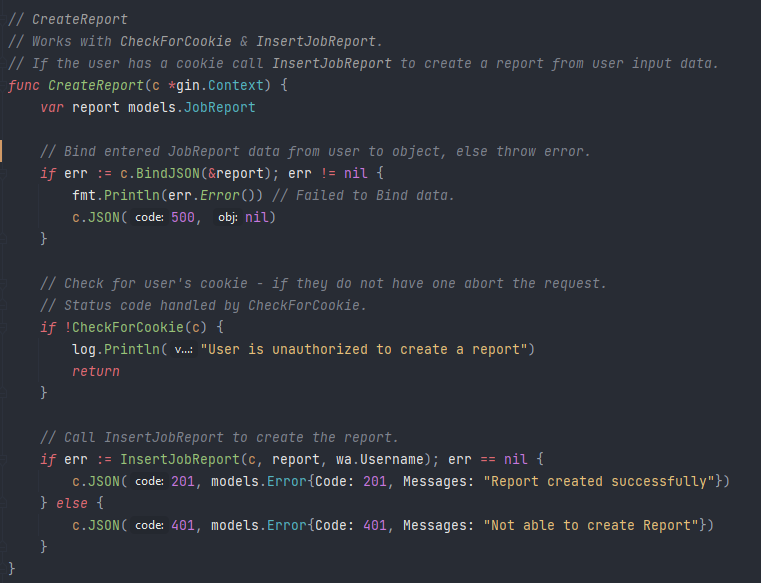
\includegraphics[width=1.0\textwidth]{images/horton/report_system/create_report.png}
\end{figure}

\begin{figure}[H]
    \caption{Prepare MySQL INSERT QUERIES}
    \label{image:insertReport}
    \centering
    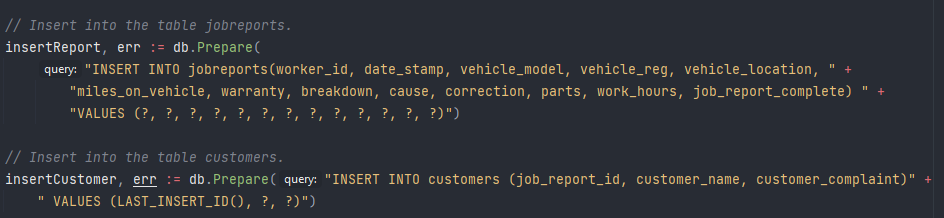
\includegraphics[width=1.0\textwidth]{images/horton/report_system/insert_report.png}
\end{figure}


\begin{figure}[H]
    \caption{Go MySQL Transaction for two INSERTs}
    \label{image:go_mysql_trans}
    \centering
    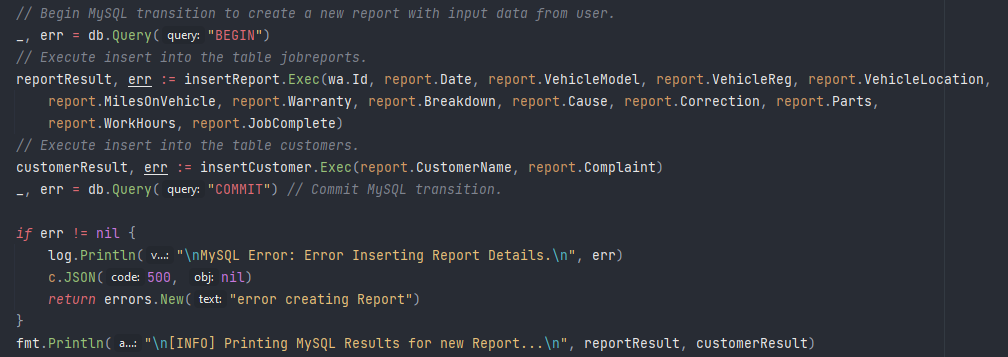
\includegraphics[width=1.0\textwidth]{images/horton/report_system/go_mysql_transaction.png}
\end{figure}

\subsubsection{Get Reports}
Retrieving reports owned by a user are handled by the functions GetReports, CheckForCookie and isValidAccount. This starts off with the client sending a GET request. The user is first checked with the functions CheckForCookie and isValidAccount (Figure 4.29). This is to ensure the user owns these reports. If they do a MySQL JOIN QUERY is initiated to select all the user's reports (Figure 4.30) in the database. The reports are then send to the client with a status code of 200 - meaning the retrieval was a Status OK.

\begin{figure}[H]
    \caption{GetReports Function}
    \label{image:getReports}
    \centering
    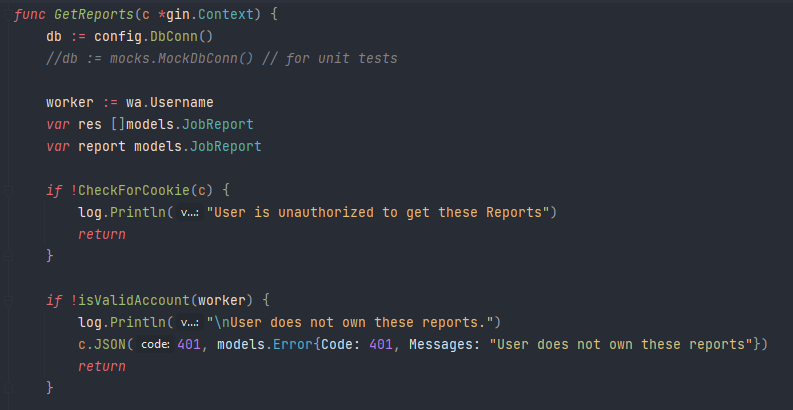
\includegraphics[width=0.78\textwidth]{images/horton/report_system/get_reports.png}
\end{figure}

\begin{figure}[H]
    \caption{Go MySQL JOIN to SELECT all Reports}
    \label{image:go_mysql_join}
    \centering
    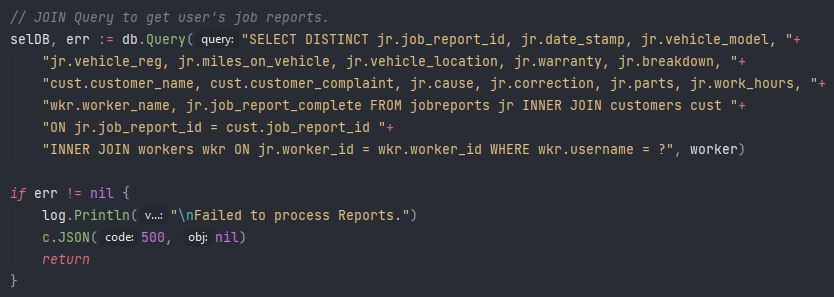
\includegraphics[width=1.0\textwidth]{images/horton/report_system/go_mysql_join.png}
\end{figure}

\subsubsection{Get A Report by ID}
GetReports and GetReportById are similar to each other. The difference being GetReports retrieves all reports owned by a user, and GetReportById gets a single report. GetReportById gets the report's ID from its parameter of the path e.g. /jobReports/ID (Figure 4.31). Retrieving a single report begins with a GET request from the client. The user is then checked the same as if they were getting all their reports. Then a MySQL JOIN QUERY is done with the requested report's ID (Figure 4.32) to select it from the database, and the report is sent to the client with a status code of 200.

\begin{figure}[H]
    \caption{ID Parameter from Report}
    \label{image:report_param_id}
    \centering
    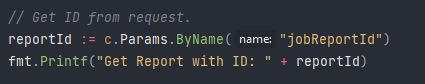
\includegraphics[width=1.0\textwidth]{images/horton/report_system/get_report_id.png}
\end{figure}

\begin{figure}[H]
    \caption{Go MySQL JOIN to SELECT a singe Report}
    \label{image:report_by_id}
    \centering
    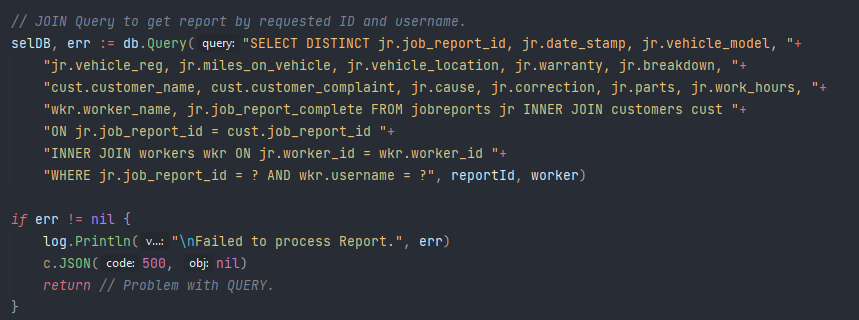
\includegraphics[width=1.0\textwidth]{images/horton/report_system/go_mysql_report_id.png}
\end{figure}

\subsubsection{Update A Report}
Updating a report starts with a PUT request from the client with the report's ID as a parameter and its changed data. The user is then checked and the report data is then bound to JSON with the JobReports model. Next, a MySQL UPDATE QUERY is done with the reports new data in the database and a status code of 202 is sent to the client to inform them it has been updated - Figure below.

\begin{figure}[H]
    \caption{Go MySQL UPDATE a Report}
    \label{image:updateReport}
    \centering
    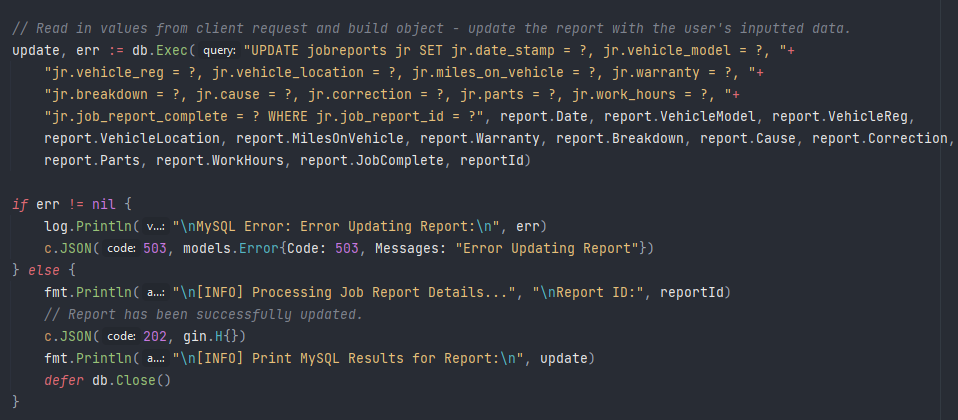
\includegraphics[width=0.8\textwidth]{images/horton/report_system/update_report.png}
\end{figure}

\subsubsection{Delete A Report}
Deleting a Report begins with a DELETE request from the client request report by its ID. The user is checked and a MySQL DELETE QUERY is executed to remove the report from the database. Then a status code of 204 (No Content) is send to the client to notify the deletion of the report was successful - Figure below. 

\begin{figure}[H]
    \caption{DeleteReport Function}
    \label{image:deleteReport}
    \centering
    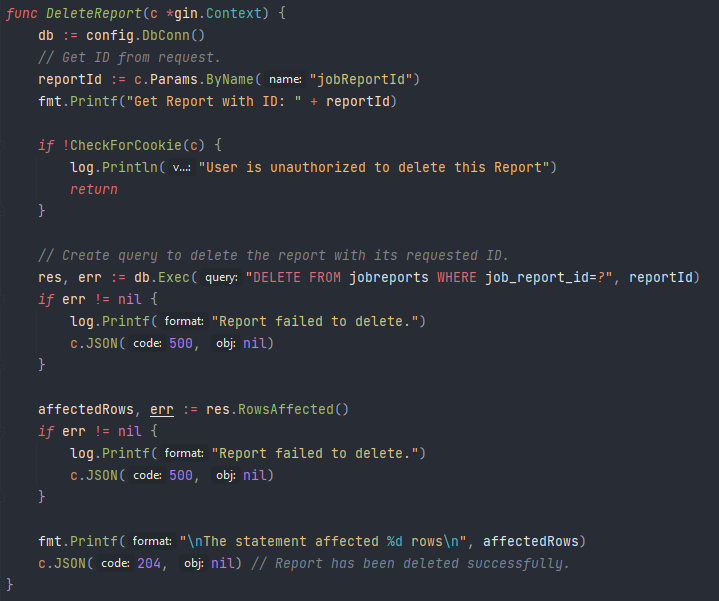
\includegraphics[width=0.6\textwidth]{images/horton/report_system/delete_report.png}
\end{figure}

Please view the figure below for an overview of how the report system works with the controllers, handler functions, HTTP methods, and paths.
\begin{figure}[H]
    \caption{Report System}
    \label{image:reportSystem}
    \centering
    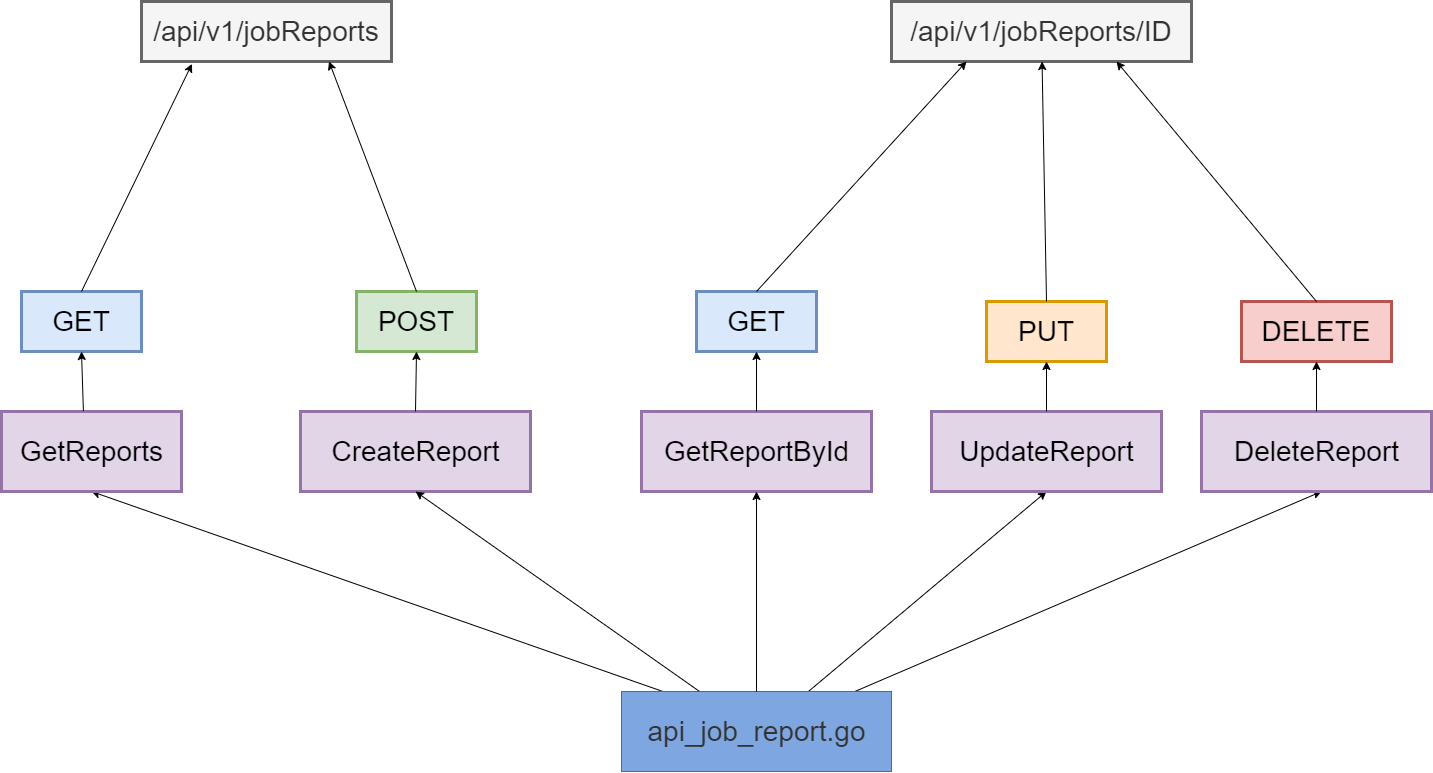
\includegraphics[width=0.8\textwidth]{images/horton/report_system/report_system.png}
\end{figure}

\subsection{3rd Party API}
The back-end has access to a 3rd Party API named Back4App which lists vehicle make and model data to make the creating and updating of reports convenient for the users. The data is gathered from the API with a GET request. Before this request is done, authorization headers are set from a configuration file to be allowed to use the API's service. After the headers are set the CheckForCookie function comes in to stop the request if the user is not logged in. This done as only the first 10k requests are free with Back4App and unauthorized users could take up all the requests. Next the GET request is done and the JSON data is decoded from the response body and sent the client with a status code 200 and the response body is closed. Figure 4.36 below shows a sample of the data from Back4App.

\begin{figure}[H]
    \caption{Back4App Vehicle Data}
    \label{image:back4app}
    \centering
    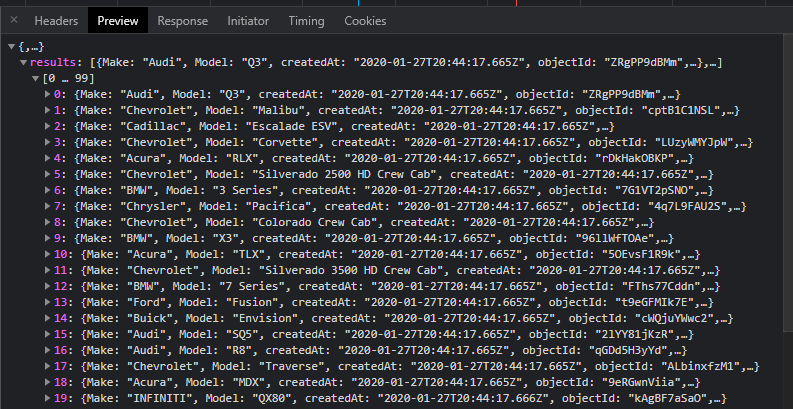
\includegraphics[width=0.8\textwidth]{images/horton/back4app/back4app_data.png}
\end{figure}

\subsection{Elastic Horton}
The back-end is hosted on AWS's Elastic Beanstalk (EB). This means it is constantly running to have it available to the front-end at all times. This process was done through the EB CLI and a Dockerfile. First, an EB environment (Figure 4.37) was set up for the back-end, then the Dockerfile was used to deploy and update the running back-end to EB. The domain name 'repota-service.com' was bought from GoDaddy. This domain was bought to have the back-end and front-end to be secure (HTTPS). A SSL certificate attached to the domain by the name of 'api.report-service.com' was acquired from AWS's Certificate Manager with the domain bought. Then the EB environment was altered to listen on port 443 for HTTPS with the SSL certificate. Route 53 was then used to point the bought domain to the EB environment. In summary, the back-end is hosted with a very secure connection (Figure 4.38).

\begin{figure}[H]
    \caption{Elastic Beanstalk Environment}
    \label{image:elasticHorton}
    \centering
    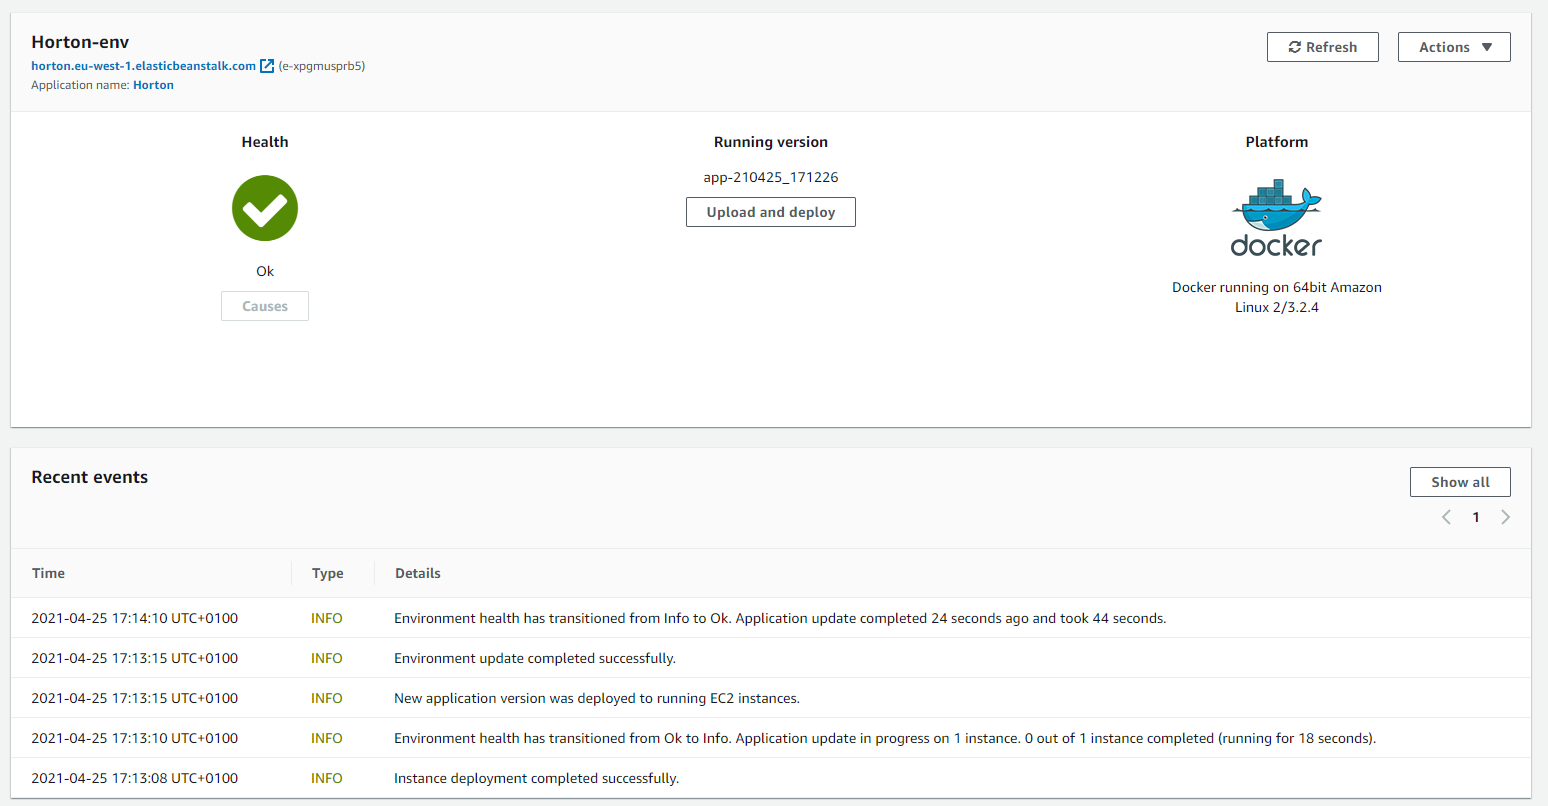
\includegraphics[width=0.8\textwidth]{images/aws/elastic_horton.png}
\end{figure}

\begin{figure}[H]
    \caption{Secure Horton}
    \label{image:secureHorton}
    \centering
    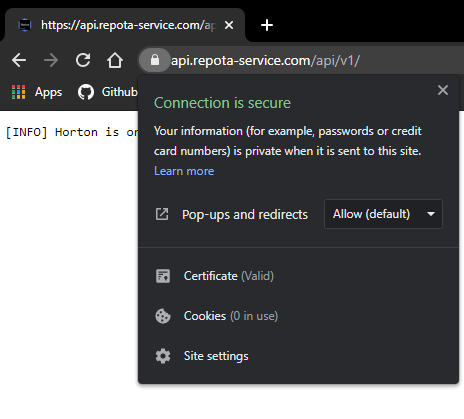
\includegraphics[width=0.5\textwidth]{images/aws/secure_horton.png}
\end{figure}

\section{The Front-end}
The front-end (Repota) is the face of it all. Repota itself was built with Angular and Ionic, while the OpenAPI specification provided the TypeScript code stubs to link Repota to Horton. The remainder of this section will explain how Repota and Horton are integrated for the users and their reports through the app's pages - Figure below.
\begin{figure}[H]
    \caption{Repota's Pages}
    \label{image:repotaPages}
    \centering
    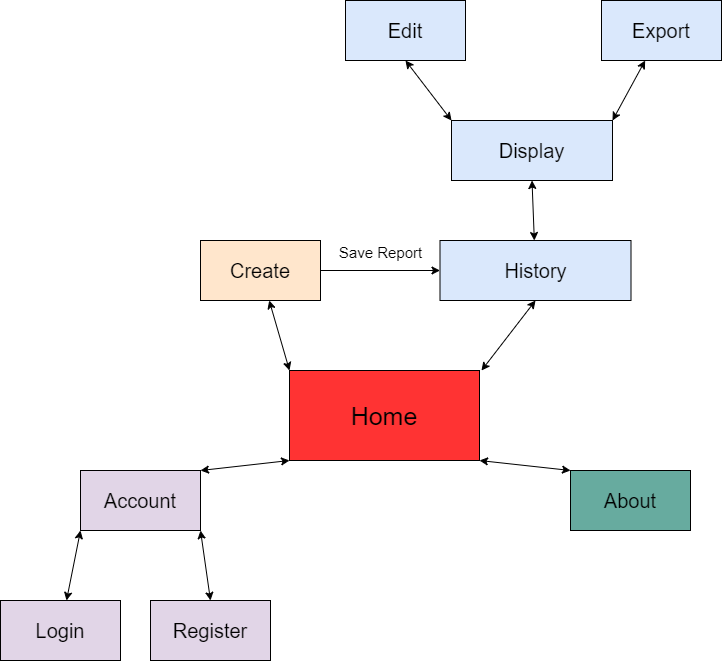
\includegraphics[width=1.0\textwidth]{images/repota/pages_diagram.png}
\end{figure}
\newpage

\subsection{Repota \& Horton Integration}
\subsubsection{Account \& Report Service}
\begin{figure}[H]
    \caption{Repota \& Horton Connection}
    \label{image:repotaNhorton}
    \centering
    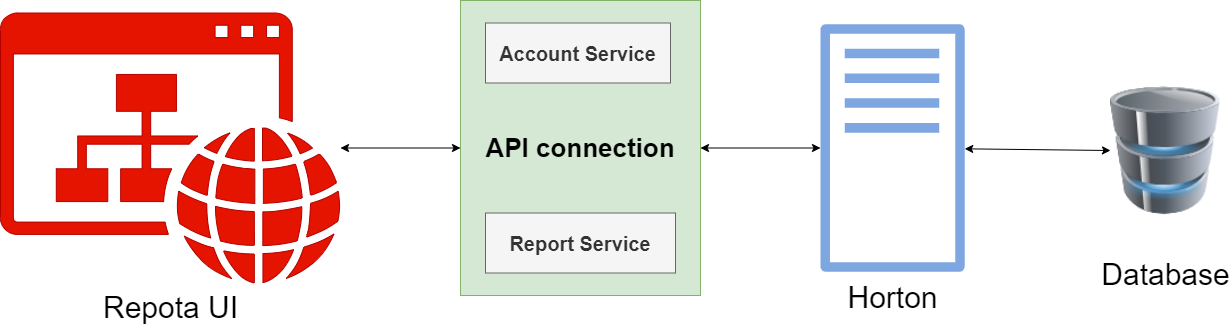
\includegraphics[width=0.8\textwidth]{images/repota_and_horton/repota_n_horton.png}
\end{figure}

The figure above displays how Repota (the front-end) is connected to Horton (API) and the database. The API connection is made through the classes AccountService and JobReportService, which came from the OpenAPI specification and required little editing. The only editing required was to change the default URL where the connection is made to the API and the addition of two methods named logout and getCarApiData - for retrieving Back4App's data from the API. AccountService handles user registration, login, and logout. AccountService is connected to API by the URL (basePath - Figure 4.41). This class allows the HTTP methods POST for register and login and GET for logout. JobReport service is similarly connected to the API to AccountService. JobReportService handles all the CRUD operations and HTTP methods: GET (Get reports \& get a report by ID), POST (Create a Report), DELETE (Delete Report), PUT (Update a Report) for reports, and retrieving Back4App's data from the API. These methods, their functionality and how they work for users will be explained below in the respected titled subsections.

\begin{figure}[H]
    \caption{Account Service Connection to API}
    \label{image:a-s-conn}
    \centering
    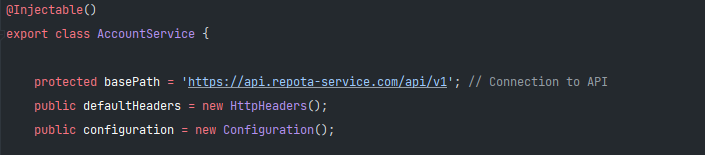
\includegraphics[width=1.0\textwidth]{images/repota_and_horton/account_service.png}
\end{figure}

\subsubsection{Model Interfaces}
The model interfaces named InLineObject and JobReport (Figures below) also came from the OpenAPI specification. These models are used for the register, login, create report and edit report forms to interact with the models with the API's models and to put the data into the database. 

\begin{figure}[H]
\centering
\begin{minipage}[b]{0.45\linewidth}
    \centering
    \caption{InLineObject Interface}
    \label{image:iloInterface}
    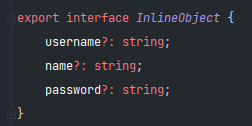
\includegraphics[width=1.0\textwidth]{images/repota/models/inlineobject_model.png}
\end{minipage}
\quad
\begin{minipage}[b]{0.45\linewidth}
    \centering
    \caption{JobReport Interface}
    \label{image:jrInterface}
    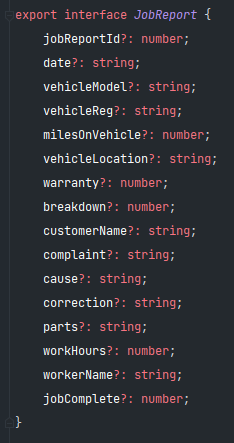
\includegraphics[width=0.8\textwidth]{images/repota/models/report_model.png}
\end{minipage}
\end{figure}

\subsection{Account Pages}

\subsubsection{Registration}
User registration is done through the Register Page. The method register (Figure 4.44) is set up as a form that uses the InLineObject model to have the user's enter details (username, name, and password) as an object to push the data with a POST request to the API with the AccountService's register method and insert the details into the database. The user must have their username at least eight characters long, their name to be their full name (as this is displayed on their reports). The password is ensured by a regular expression on the HTML side to have at least eight characters, one uppercase and lowercase letter, one number, and a special character to provide extra security (Figure 4.45). Once the user has the form filled out, they click the register button on the UI to send the data, and once the data in the database, the user is navigated to the login page. If there are errors with the registration process (e.g., the username is already taken), an error message is displayed on the UI to the user (Figure 4.46).

\begin{figure}[H]
    \caption{Register Method}
    \label{image:registerMethod}
    \centering
    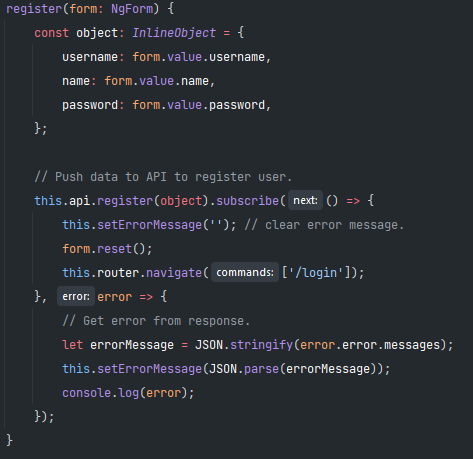
\includegraphics[width=1.0\textwidth]{images/repota/account_pages/register.png}
\end{figure}

\begin{figure}[H]
    \caption{Regular Expression pattern for Password}
    \label{image:passwordRegEx}
    \centering
    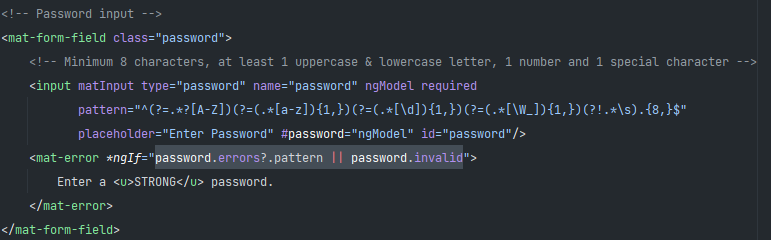
\includegraphics[width=1.0\textwidth]{images/repota/account_pages/password_regex.png}
\end{figure}

\begin{figure}[H]
    \caption{Username is already taken - Error}
    \label{image:nameTaken}
    \centering
    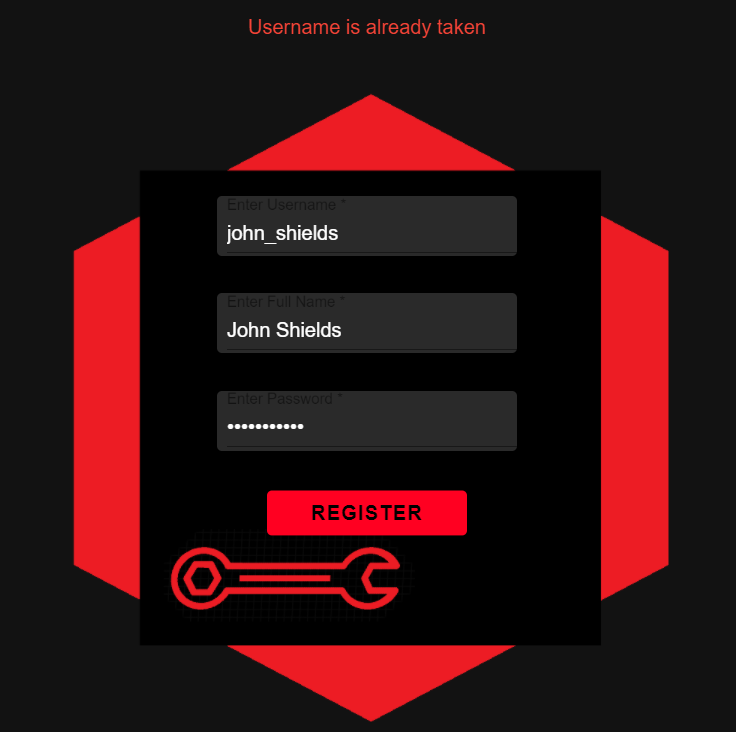
\includegraphics[width=0.5\textwidth]{images/repota/UI/username_taken.png}
\end{figure}

\subsubsection{Login}
User login is managed on the Login Page. This process is handled by the login method (Figure 4.47). Similar to register, login is set up as a form and uses the InLineObject model. The user's entered username and password are attached to the model. Once the user clicks the login button, the data is sent to the API by a POST request through the AccountService's login method. The entered data by the user is then checked with the user's details in the database. If the information is correct, a cookie is set for three days for the user and then they are navigated to the home page. If there is a problem or the information is not correct, an error message is displayed for the user (Figure 4.48). 

\begin{figure}[H]
    \caption{Login Method}
    \label{image:loginMethod}
    \centering
    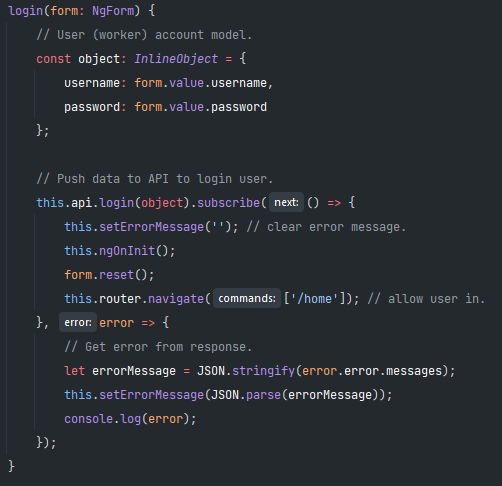
\includegraphics[width=0.55\textwidth]{images/repota/account_pages/login.png}
\end{figure}

\begin{figure}[H]
    \caption{Password is incorrect - Error}
    \label{image:failedLogin}
    \centering
    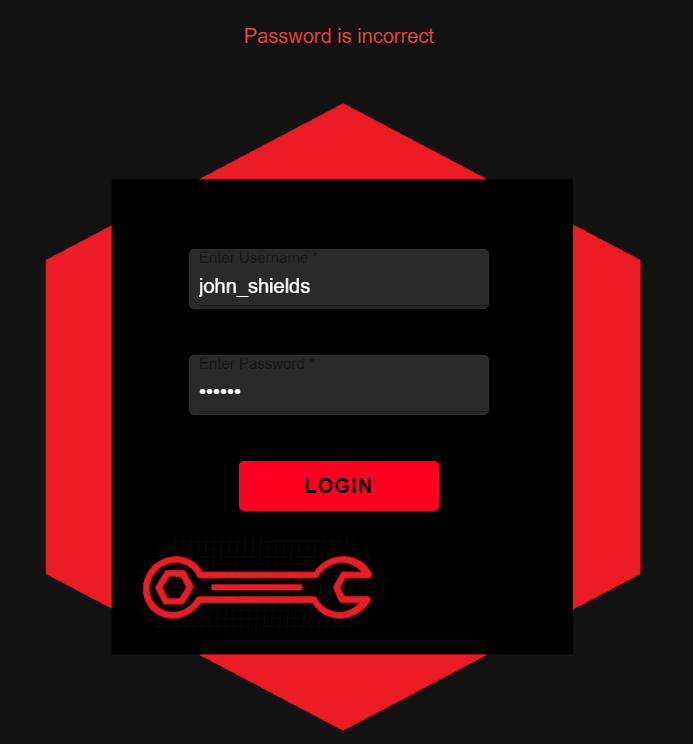
\includegraphics[width=0.5\textwidth]{images/repota/UI/failed-login.png}
\end{figure}

\subsubsection{Logout}
Logout is available to a logged-in user on any page of the front-end. The logout button is available to users in the hamburger menu (Figure 4.49). When a user clicks on the logout button, this calls the logout method (Figure 4.50). That method then sends a GET request with the AccountService's logout method to the API, and after one second, the user is officially logged out and navigated to the account page. The wait for one second is to allow the logged-out cookie set by the API to expire; therefore, the user does not send the logout request multiple times within that one second.

\begin{figure}[H]
    \caption{Hamburger Menu - Logout Button}
    \label{image:logoutButton}
    \centering
    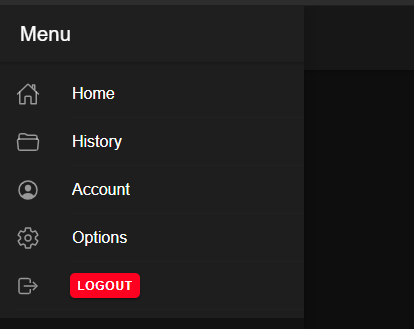
\includegraphics[width=0.5\textwidth]{images/repota/UI/logout.png}
\end{figure}

\begin{figure}[H]
    \caption{Logout Method}
    \label{image:logoutMethod}
    \centering
    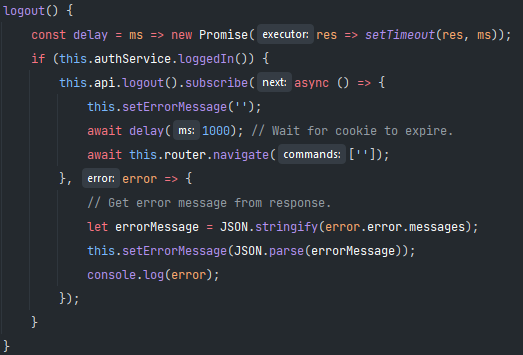
\includegraphics[width=0.6\textwidth]{images/repota/account_pages/logout_method.png}
\end{figure}

\subsection{Report Pages}

\subsubsection{History}
The History Page displays all the reports owned by a user. Only the report's number (ID), date, customer name, and the complete box are displayed here (Figure 4.51). The reports are loaded in from the API by the JobReportService's getReports method. The method ngOnInit (Figure 4.52) calls getReports from JobReportService, and the reports are automatically loaded for the user when they navigate to this page from a ngFor on the HTML side. If the user does not have any reports, a message is displayed to notify them (Figure 4.53). 

\begin{figure}[H]
    \caption{History Page}
    \label{image:historyPage}
    \centering
    \includegraphics[width=1.0\textwidth]{images/repota/UI/history-page.png}
\end{figure}

\begin{figure}[H]
    \caption{ngOnInit Method - Load all user's Reports}
    \label{image:get_reports}
    \centering
    \includegraphics[width=0.8\textwidth]{images/repota/report_pages/get_reports.png}
\end{figure}

\begin{figure}[H]
    \caption{User has no Reports}
    \label{image:noReports}
    \centering
    \includegraphics[width=0.8\textwidth]{images/repota/UI/no_reports.png}
\end{figure}

\subsubsection{Display}
The Display Page shows a single report. A user can see the report by clicking the open button on a report from the history page. This button navigates the report with the selected report's ID as a parameter to the display page. The full data of the report is displayed here by a ngFor with the options to edit, export it to a PDF and delete (Figure 4.54). The report is loaded by the ngOnInit method (Figure 4.55) and from the API through the JobReportService's getReportById method. If the ID parameter is not the ID for a report in the database or the user does not own the report, a 'Report not found' message is displayed (Figure 4.56).  

\begin{figure}[H]
    \caption{Display Page}
    \label{image:displayPage}
    \centering
    \includegraphics[width=1.0\textwidth]{images/repota/UI/display-page.png}
\end{figure}

\begin{figure}[H]
    \caption{ngOnInit Method - Get Report by ID}
    \label{image:ng_reportbyID}
    \centering
    \includegraphics[width=1.0\textwidth]{images/repota/report_pages/display.png}
\end{figure}

\begin{figure}[H]
    \caption{Report not found}
    \label{image:ReportNotFound}
    \centering
    \includegraphics[width=1.0\textwidth]{images/repota/UI/report_not_found.png}
\end{figure}

\subsubsection{Create}
Users construct their reports through a form on the Create page. The method createReport uses the JobReport model as an object for all the data the user enters (Figure 4.57). The values, warranty, breakdown, and complete are checkboxes. These values required lists to input the data along with an if/else statement to turn the check box values from true and false to 1 and 0 (Figure 4.58). This alteration is to accommodate the values on the Go side of the model and the database. Once the user has entered the report's information and clicks the create button, this data gets sent through a POST request to the API through the JobReportService. After the report is in the database, the user is navigated to the history page. The data from Back4App is loaded in though the ngOnInit method (Figure 4.59) from the API and is displayed to the user as a HTML data list (Figure 4.60).  

\begin{figure}[H]
    \centering
    \caption{JobReport Object \& Push Object to API}
    \includegraphics[width=0.65\textwidth]{images/repota/report_pages/create_2.png}
    \label{image:createReportObject}
    \centering
\end{figure}

\begin{figure}[H]
    \centering
    \caption{Checkboxes - If/Else Statement}
    \label{image:createReportIf-Else}
    \includegraphics[width=0.8\textwidth]{images/repota/report_pages/create_1.png}
\end{figure}

\begin{figure}[H]
    \centering
    \caption{ngOnInit method - Back4App Data}
    \label{image:ngOnInitBack4App}
    \includegraphics[width=0.8\textwidth]{images/repota/report_pages/back4app.png}
\end{figure}

\begin{figure}[H]
    \centering
    \caption{Create Page - HTML data list}
    \label{image:HTMLdatalist}
    \includegraphics[width=1.0\textwidth]{images/repota/UI/create-data.png}
\end{figure}

\subsubsection{Edit}
Users can make changes or complete their reports on the Edit Page. They can access the edit page from the display page by clicking the edit button on the report. This carries over the report's ID to the edit page. The report's data is available through the loadReportById method (Figure 4.61) in HTML data lists (Figure 4.62). This setup was an improvise as when the data was loaded straight into the input boxes, it was unchangeable, and users would still have to retype it all. If the data were loaded into an input box, there would be two inputs updated in the database. For example, the 'Make \& Model' box would have the value 'Ford Focus', and the user types in 'Ford Focus' again and submitted the edit. In the database, the value would be 'Ford Focus Ford Focus'. This method was not suitable. The HTML data list solved this problem as the user only has to click the data to have it in the input box again.

\begin{figure}[H]
    \centering
    \caption{loadReportById Method}
    \label{image:loadReportById}
    \includegraphics[width=0.8\textwidth]{images/repota/report_pages/load_report.png}
\end{figure}

\begin{figure}[H]
    \centering
    \caption{Edit Page - HTML data list}
    \label{image:EditHTMLdatalist}
    \includegraphics[width=1.0\textwidth]{images/repota/UI/edit-page.png}
\end{figure}

Similar to the create page, the Back4App's data is retrieved from the API to the Make \& Model input box. The only difference is that the request is made through the method loadCarData and, along with loadReportById, are called in ngOnInit. This abstraction was done to ensure code quality and performance. Initially, all the code for retrieving Back4App's and the report's data, along with the lists for the checkboxes, was in the ngOnInit method. The checkboxes' structure is in relation the the create page's structure for them.

The user submits the edit with the edit button. This submission calls the editReport method and correspondent with the createReport method. editReport uses the JobReport model as an object with the report's altered data and calls the updateReport method from JobReportService with a PUT request to the API. This process updates the report in the database and navigates the user back to the history page.

\subsubsection{Export}
Users can export their reports to PDFs from the Export Page. Exporting reports is accessed on the display page of a report by the PDF button. When a user clicks on this button, the report is brought and load over by its ID through the ngOnInit method from the API on the export page. The export page presents the report in a printable format (Figure 4.63). When a user clicks on the Export PDF button, this calls the method onExportPDF (Figure 4.64), which brings up a file explore window for the user to save the report locally. onExportPDF uses the libraries dom-to-image and jsPDF. dom-to-image converts the HTML DOM (Document Object Model) to a PNG image, then this image is added to a PDF made by jsPDF. Next, the report is saved to a file named service\_report.pdf (Figure 4.65).

\begin{figure}[H]
    \centering
    \caption{Export Page}
    \label{image:export}
    \includegraphics[width=1.0\textwidth]{images/repota/UI/export-page.png}
\end{figure}

\begin{figure}[H]
    \centering
    \caption{onExportPDF Method}
    \label{image:onExportPDF}
    \includegraphics[width=1.0\textwidth]{images/repota/report_pages/export.png}
\end{figure}

\begin{figure}[H]
    \centering
    \caption{Service Report PDF}
    \label{image:reportPDF}
    \includegraphics[width=1.0\textwidth]{images/repota/service_report_pdf.png}
\end{figure}

\subsubsection{Delete}
The deletion of a report is handled on the display page. When a user clicks the delete option, a popup box displays asking them are they sure to delete it (Figure 4.66). When the user clicks 'OK' on the popup box, the method deleteReport (Figure 4.67) is called to send a DELETE request to the API through the JobReportService with the corresponding method. Once the request is complete, the report is removed from the database, and the user is navigated back to the history page.

\begin{figure}[H]
    \centering
    \caption{Delete Report Confirmation}
    \label{image:deleteReportConfirm}
    \includegraphics[width=0.85\textwidth]{images/repota/UI/confirm-delete.png}
\end{figure}

\begin{figure}[H]
    \centering
    \caption{deleteReport Method}
    \label{image:deleteReportMethod}
    \includegraphics[width=0.8\textwidth]{images/repota/report_pages/delete.png}
\end{figure}

\subsubsection{Error Messages}
All error messages for user registration, login, and logout, along with the CRUD operations for reports, are handled with getters and setters (Figure 4.68). As shown and discussed above, error messages are displayed for invalid user inputs and 404s (Not found errors). Any errors from the API are extracted into a string format and then set as the parsed message to the setter (Figure 4.69). The getter is then used on the HTML side to display the error to the user, as shown above. These errors can also let users know of any serious errors from the API. For instance, an error with the status code 500 (Internal Server Error) if a request went horribly wrong on the API's side. For example, an internal server error could be a failure to process a request, and the users must be notified immediately to avoid confusion.

\begin{figure}[H]
    \centering
    \caption{Error Message Handlers}
    \label{image:errorMessageHandlers}
    \includegraphics[width=0.6\textwidth]{images/repota/report_pages/error_handlers.png}
\end{figure}

\begin{figure}[H]
    \centering
    \caption{JSON extracting \& parsing of error message}
    \label{image:letError}
    \includegraphics[width=0.8\textwidth]{images/repota/report_pages/let_error.png}
\end{figure}

\subsection{AuthGuard}
When an unauthorized user visits Repota the pages home, history, display, create, edit, export are blocked. If the user tries to navigate to the home page through the hamburger menu the error message 'Please login first' displays (Figure 4.70). Also the history page and logout button are also not available. This security is a result of the AuthGuard implementation into the app. The AuthGuard blocks pages to users that do not have cookies (unauthorized users). The classes AuthGaurd and AuthService work together. AuthService uses the method loggedIn (Figure 4.71) to check if a user has a cookie or not. If the user is not logged in a boolean is set as false with the method canActivate (Figure 4.72) in the AuthGaurd class. canActivate is then used in the class AppRoutingModule to block the pages listed above (Figure 4.73).

\begin{figure}[H]
    \centering
    \caption{Please login first}
    \label{image:pleaseLogin}
    \includegraphics[width=0.6\textwidth]{images/repota/UI/please_login.png}
\end{figure}

\begin{figure}[H]
    \centering
    \caption{loggedIn Method}
    \label{image:loggedIn}
    \includegraphics[width=0.8\textwidth]{images/repota/auth_guard/loggedIn.png}
\end{figure}

\begin{figure}[H]
    \centering
    \caption{canActivate Method}
    \label{image:canActivate}
    \includegraphics[width=0.9\textwidth]{images/repota/auth_guard/can_activate.png}
\end{figure}

\begin{figure}[H]
    \centering
    \caption{Blocked Routes}
    \label{image:blocked}
    \includegraphics[width=0.9\textwidth]{images/repota/auth_guard/blocked_routes.png}
\end{figure}

As mentioned above, when a user logs in, they receive a cookie. Once they are logged in, all the pages are unblocked, and they are free to explore the app through the hamburger menu. The method loggedIn is used throughout the app with Angular's ngIf to disable the login and register if a user is already logged in/registered. Suppose a user is logged in and navigates to the login or register page a message displays to notify them that they are already authorized (Figure 4.74). 

\begin{figure}[H]
    \centering
    \caption{Already logged in message}
    \label{image:alreadyLoggedIn}
    \includegraphics[width=0.8\textwidth]{images/repota/UI/already_loggedIn.png}
\end{figure}

\subsection{Repota UI}
Throughout this chapter, a majority of Repota's UI has been shown. This section will go through the UI pages Home, Account, and About. As seen on the login and register page, the app's logo is used throughout these pages to provide consistency and an iconic style. When a user logs in, they are navigated to the home page. There are two buttons to navigate to the pages create and history (Figure 4.75). The about page (Figure 4.76) can be accessed and navigated to through the hamburger menu. This page displays a short description of the app and two buttons as hyperlinks for the app's guide located at the project's Wiki of the GitHub repository and the repository itself. The initial visiting page of the app is the account page (Figure 4.77). When a user is not logged in, a welcome message is displayed, controlled by the loggedIn method from the AuthService class. The buttons on the page provide navigation to the pages login and register. 

\begin{figure}[H]
    \centering
    \caption{Home Page}
    \label{image:homePage}
    \includegraphics[width=0.8\textwidth]{images/repota/UI/home-page.png}
\end{figure}

\begin{figure}[H]
    \centering
    \caption{About Page}
    \label{image:aboutPage}
    \includegraphics[width=0.8\textwidth]{images/repota/UI/about.png}
\end{figure}

\begin{figure}[H]
    \centering
    \caption{Account Page}
    \label{image:accountPage}
    \includegraphics[width=0.8\textwidth]{images/repota/UI/account.png}
\end{figure}

\subsection{Repota Bucket}
Repota is hosted on AWS's S3 bucket. This procedure was reached through the AWS S3 CLI. The app was built for production using the Angular command 'ng build --prod'. The production directory was then deployed to S3 Bucket. Resembling Horton, Repota is also HTTPS. This process was achieved through AWS's Route 53, CloudFront, and Certificate Manager. The bought domain from GoDaddy was set to 'www.repota-service.com' through AWS's Route 53 to point to the bucket. Then the SSL certificate was retrieved from the Certificate Manager. CloudFront was then used to have the bucket attach to the SSL certificate. Resulting in Repota being secure (Figure below).

\begin{figure}[H]
    \centering
    \caption{Secure Repota}
    \label{image:secureRepota}
    \includegraphics[width=0.8\textwidth]{images/aws/secure_repota.png}
\end{figure}